\documentclass[xcolor={dvipsnames},pdf, hyperref={colorlinks=true, citecolor=ForestGreen, linkcolor=BlueViolet, urlcolor=Magenta}]{beamer}
\usetheme{Frankfurt}  
\usecolortheme{whale}
\usepackage{tikz} 
\usepackage{amsmath}
\usepackage{amsthm}
\usepackage{amssymb}              % used for \eqref{} in this document
\usepackage{dsfont}
\usepackage{hyperref}
\usepackage{threeparttable}
\usepackage{multirow}
\graphicspath{{Figures/}}
\usepackage{booktabs}
\newtheorem{exmp}{Example}[section]
\usepackage{subcaption}
\usepackage{adjustbox}
\usepackage{graphicx}
\usepackage[mathscr]{euscript}
\usepackage{remreset}% tiny package containing just the \@removefromreset command
\makeatletter
\@removefromreset{subsection}{section}
\makeatother
\setcounter{subsection}{1}
\usepackage{float}
\usepackage{sgamevar}
\usepackage{sgame}


\newcommand{\defn}[1]{\textbf{#1}}


%Instructor version
\newcommand{\blank}[0]{}
\newcommand{\ddp}[1]{{\textcolor{ForestGreen}{#1}}} 
\newcommand{\dd}[1]{{\underline{\textcolor{ForestGreen}{#1}}}}

%Student version
%\newcommand{\blank}[0]{\vspace{2em}}
%\newcommand{\dd}[1]{\underline{\hspace{3cm}}} 
%\newcommand{\ddp}[1]{}

\addtobeamertemplate{navigation symbols}{}{%
	\usebeamerfont{footline}%
	\usebeamercolor[fg]{footline}%
	\hspace{1em}%
	\insertframenumber/\inserttotalframenumber
}

\section{Introduction}

%% preamble
\title{Monopoly}
\author{David A. D\'iaz}
\institute{UNC Chapel Hill}
\date{}


\AtBeginSection[] %Section links on slides


\begin{document} 
	
	\begin{frame}
		
		\titlepage
		
	\end{frame}



\begin{frame}{Monopoly}
\begin{itemize}
	\item \defn{Monopoly:} A fire that is the sole seller of a product without close substitutes.
	\item 	Monopolies arise due to lack of competition and thus have a great deal of market power. In contrast to perfectly competitive firms, monopolies are \dd{price makers}.
	\item Fundamental cause: barriers to entry
\end{itemize}
\end{frame}

\begin{frame}{Monopoly}
	\begin{itemize}
		\item Barriers to entry:
			\begin{enumerate}
			\item Monopoly Resources: A key resource required for production is owned by a single firm.
			\item Government-Created Monopolies: The gov. gives a single firm the exclusive right to produce some good or service.
			\item \defn{Natural Monopolies}: A monopoly that arises because a single firm can supply a good or service to an entire market at a smaller cost than could two or more firms. \textit{Experiences economies of scale over the relevant range of output}.
			\end{enumerate}
	\end{itemize}

\end{frame}

\begin{frame}[b]{Monopoly}
	\begin{figure}[H]
	\centering
	\ddp{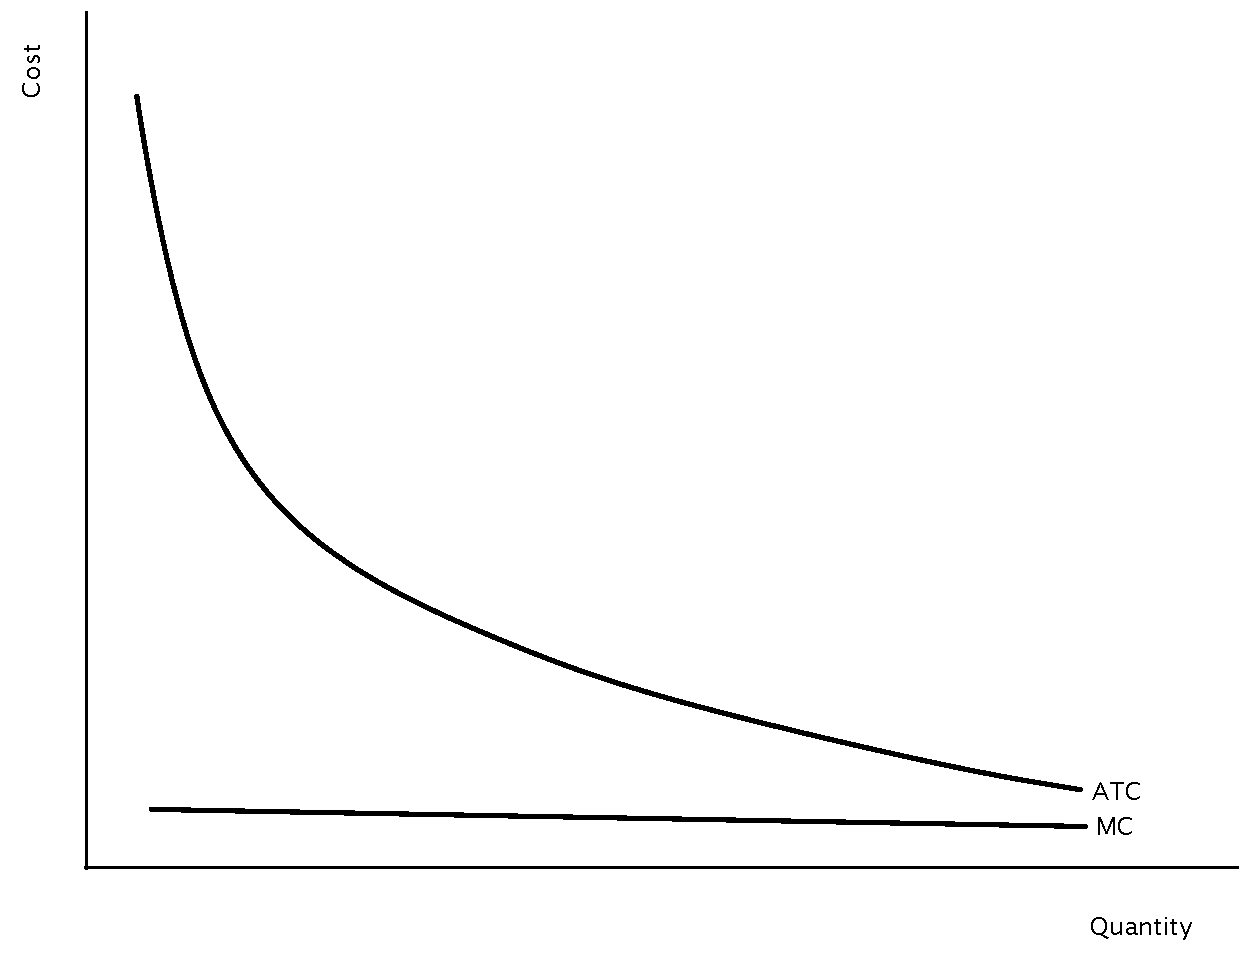
\includegraphics[scale=.40]{plot74.pdf}}
	\caption{Natural Monopoly Cost Curves}
\end{figure}
\end{frame}

\section{Production Decisions}

\begin{frame}{Production Decisions}
\begin{itemize}
	\item In contrast to firms in perfect competition, which have a \dd{horizontal demand} due to the goods being perfect substitutes, a monopoly's demand curve is the \dd{market} demand curve. 
	\item This demand curve is \dd{downward sloping} -- as the price the monopoly charges increases, the quantity demanded of the good decreases.

\end{itemize}
\end{frame}

\begin{frame}{Production Decisions}
	\begin{itemize}
		\item The monopoly thus has to balance two effects on total revenue when it increases or decreases the amount it sells:
		
		\begin{enumerate}
			\item The output effect: Increasing (decreasing) output tends to increase (decrease) total revenue.
			\item The price effect: Falling (rising) price increases (decreases) total revenue.
		\end{enumerate}
		
	\end{itemize}
\end{frame}


\begin{frame}{Production Decisions}
	\begin{exmp} \scriptsize Suppose a monopolist faces the demand schedule in Table \ref{mono}. Calculate the total revenue the firm can obtain at each price and the MR for each quantity.
	
	\begin{table}[ht]
		\centering
		\caption{Demand Schedule}
		\label{mono}
		\begin{tabular}{ c|c|c|c}        
			
			Price & Quantity & TR & MR  \\
			\hline
			\$21 & 0 &  \ddp{0}&  \ddp{---} \\
			\$20 & 1 & \ddp{21}& \ddp{21}\\
			\$19 & 2 & \ddp{38}& \ddp{17}\\
			\$18 & 3 & \ddp{54}& \ddp{16}\\
			\$17 & 4 & \ddp{68}& \ddp{14}\\
			\$16 & 5 & \ddp{80}& \ddp{12}\\
			\$15 & 6 & \ddp{90}& \ddp{10}\\
			\$14 & 7 & \ddp{98}&  \ddp{8}\\
			\$13 & 8 & \ddp{104}&  \ddp{6}\\
		\end{tabular}
	\end{table}
\end{exmp} 
\end{frame}


\begin{frame}{Profit Maximization}
	\begin{itemize}
		\item Just like firms in perfect competition, the monopolist will choose the level of output where \dd{$MR = MC$}. 
		\item 	However, in the case of perfectly competitive firms we had that \dd{$P = MR$}. 
		\item But in the case of monopolies, it is the case that \dd{$P > MR$}. 
	\end{itemize}
\end{frame}

\begin{frame}{Profit Maximization}
	\begin{itemize}
		\item After choosing the optimal quantity to produce, the price the monopoly will charge is found by tracing up from this optimal quantity up to the \dd{demand curve}.
		\item Importantly, this implies that the price a monopolist charges is \dd{greater than} the marginal cost at that quantity. This difference is called the \dd{mark-up}, $\mu = $ \dd{$P - MC(Q^*)$}.
	\end{itemize}
\end{frame}

\begin{frame}[b]{Profit Maximization}
	\begin{figure}[H]
	\centering
	\ddp{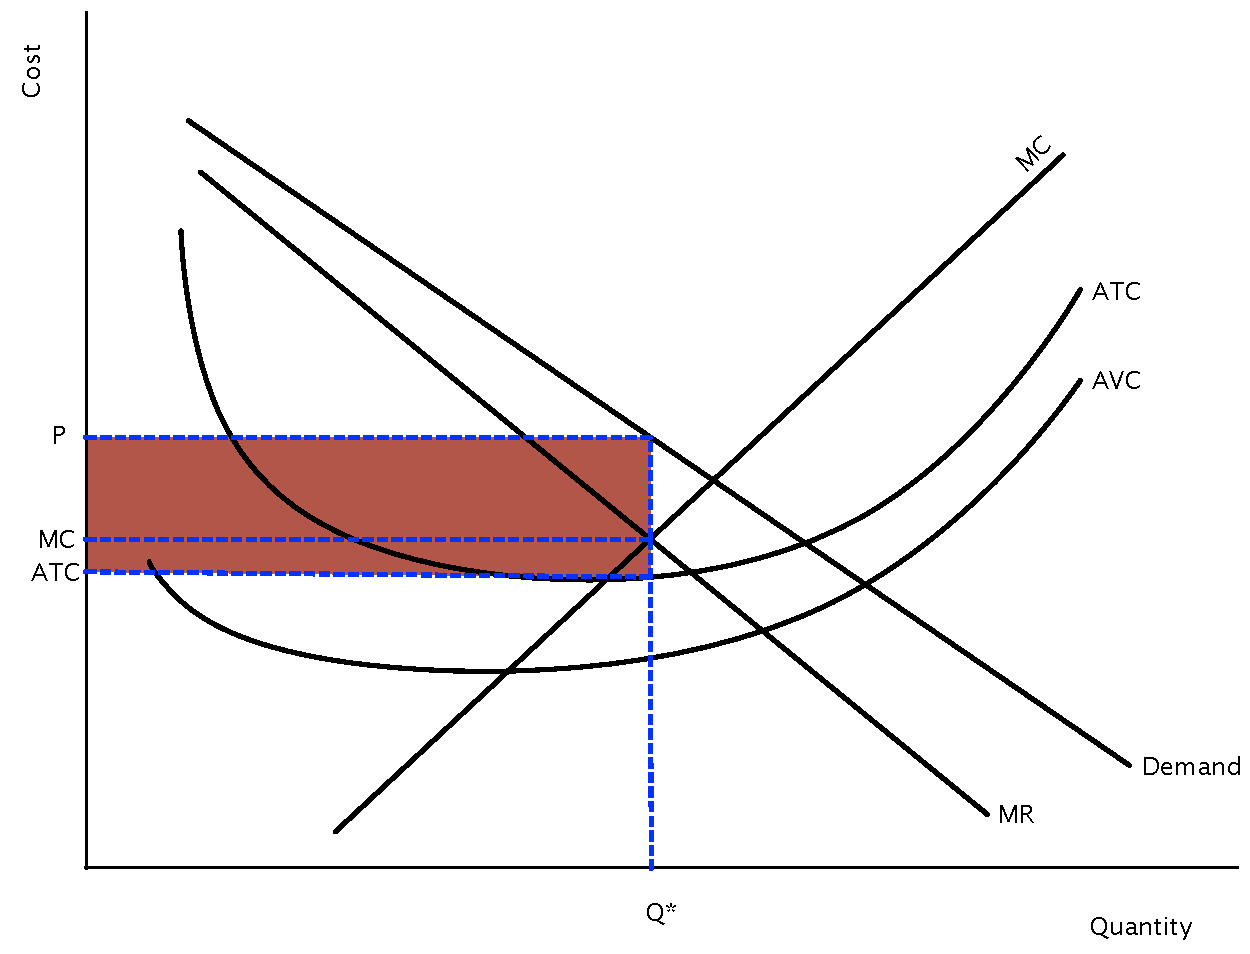
\includegraphics[scale=.40]{plot75.pdf}}
	\caption{Monopolist Environment}
\end{figure}
\end{frame}

\begin{frame}{Profit Maximization}
	\begin{exmp}
	Suppose the monopolist in Example 11.1 has constant $MC=\$10$/unit and $FC$ = \$20. What is the optimal quantity for the monopolist to produce? What price will the monopolist charge? What is the mark-up? What will its profit be?
\end{exmp}
\pause \ddp{If MC=\$10, monopolist will produce 6 units and charge a price of \$15. \\ 
	The mark-up over the marginal cost is \$5. \\
	VC of producing 6 units = \$60 since MC is constant \$10. $\Pi = 90 - (60 + 20) = \$10$.}
\end{frame}

\section{Welfare Considerations}

\begin{frame}{Welfare Considerations}
\begin{itemize}
	\item 	A monopolist charges a price above marginal cost. For consumers, this higher price diminishes their surplus. 
	\item But the firm itself gains surplus by being able to charge this higher price. From a social efficiency stand point, is the quantity that monopolies sell at the one that maximizes total surplus?
	\item Since the marginal cost curve of the monopolist reflects the costs of production, we see that the socially optimal quantity to produce is where $MC$ equals \dd{demand}.
\end{itemize}

\end{frame}

\begin{frame}[b]{Welfare Considerations}
	\begin{figure}[H]
	\centering
	\ddp{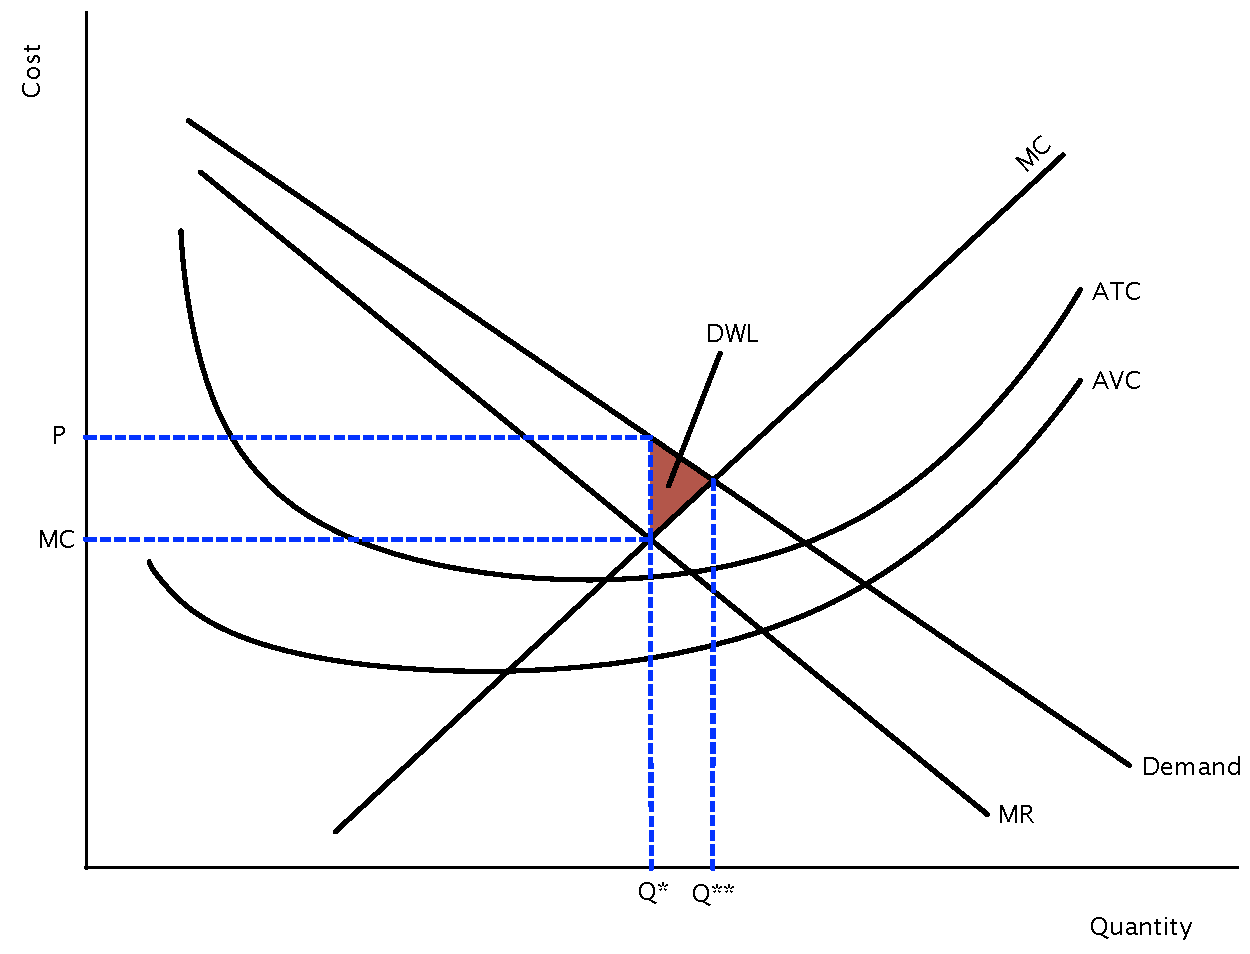
\includegraphics[scale=.35]{plot76.pdf}}
	\caption{Monopolists and Welfare}
\end{figure}
\end{frame}

\begin{frame}{Welfare Considerations}
\begin{itemize}
	\item 	This is efficient because at quantities below $Q^{**}$, the value to buyers is \dd{greater} than the cost to the monopolist. 
	\item At quantities above $Q^{**}$, the value to buyers is \dd{less} than the cost to the monopolist.
	\item Therefore, to achieve the efficient outcome the price that should be charged is where the demand curve and the marginal cost curve intersect. 
\end{itemize}
\end{frame}

\begin{frame}{Welfare Considerations}
	\begin{itemize}
	
		\item That is, just like in the case of perfect competition, the socially efficient quantity is given by where \dd{$P = MC$}. 
		\item However, a monopolist will produce \dd{less than} the socially efficient quantity due to the mark up over marginal cost.
	\end{itemize}
\end{frame}

\section{Price Discrimination}

\begin{frame}{Price Discrimination}
\begin{itemize}
	\item 	\defn{Price Discrimination:} The practice of selling the same good at different prices to different customers.
	
	\begin{enumerate}
		\item A price-discriminating monopolist can charge each consumer a price closer to their willingness to pay. 
		\item This, in turn, allows the monopolist to increase its profits.
		\item In order to price discriminate, the monopolist has to be able to separate consumers by their willingness to pay (e.g., age, geographic region, etc.).
		\item By bringing more consumers into the market, price discrimination potentially increases economic welfare.
	\end{enumerate}
	\item In the situation where the monopolist can perfectly price discriminate, then the monopolist will charge each person exactly their willingness to pay and the monopolist gets the entire surplus. 
\end{itemize}
\end{frame}

\begin{frame}{Price Discrimination}
\begin{itemize}
	\item If we simplify our graph so that $MC = ATC$ and is constant (i.e., constant per unit costs), we can easily see how this increases total surplus:
	
	\blank \blank \blank \blank
	\begin{figure}[H]
		\centering
	\ddp{	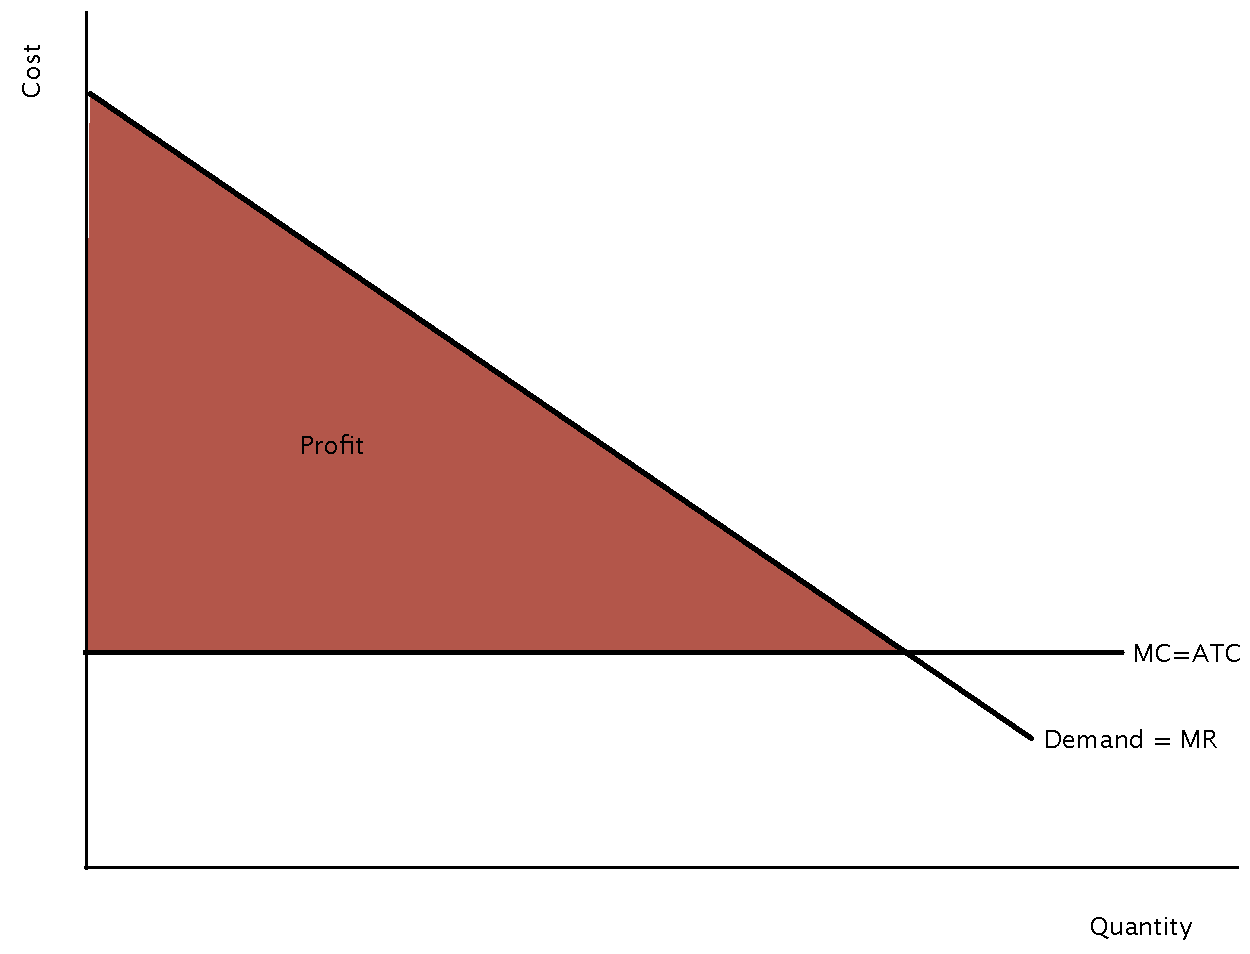
\includegraphics[scale=.2]{plot77.pdf}}
		\caption{Perfect Price Discrimination}
	\end{figure}
	\item When price discrimination is imperfect, as it usually is, the general effect on total welfare is ambiguous. However, it is always true that price discrimination allows a monopolist to increase its profits.
	
\end{itemize}
\end{frame}

\begin{frame}{Price Discrimination}
	\begin{itemize}
		\item 	Because monopolies do not produce the socially efficient quantity, policymakers attempt to respond to this issue in several ways.  
		
		\begin{enumerate}
			\item Increasing competition (e.g., antitrust laws)
		
			
			\item Public ownership (i.e., government runs monopoly itself)
			\item Doing nothing
		\end{enumerate}
	\end{itemize}
\end{frame}

\begin{frame}{Price Discrimination}

		\begin{enumerate}
		\setcounter{enumi}{3}
			\item Regulation 
			
			\begin{figure}[H]
				\centering
				\caption{Price Regulation}
				\begin{subfigure}{.4\textwidth}
					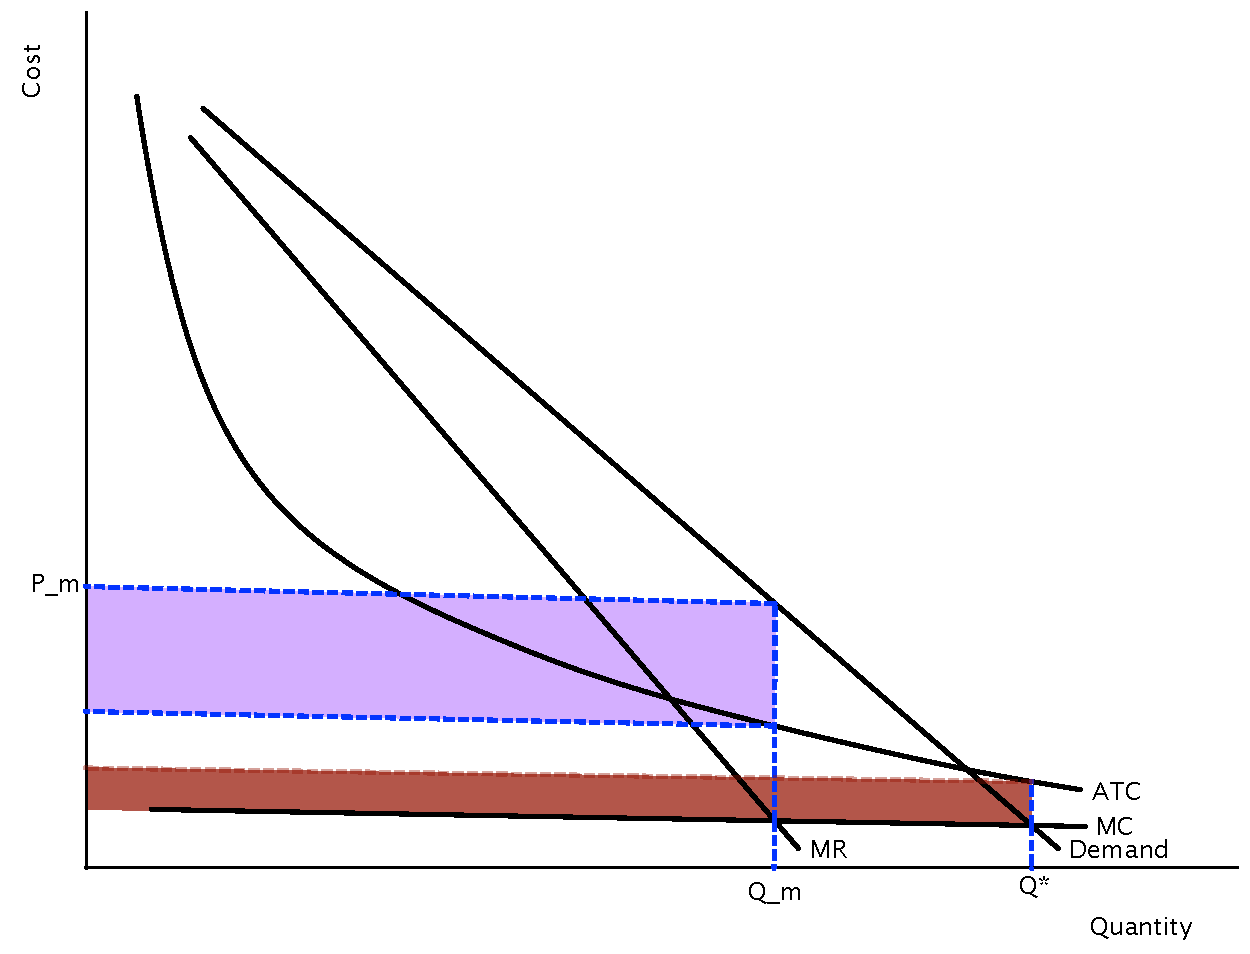
\includegraphics[scale=.18]{plot78.pdf}
					\caption{MC Pricing}
				\end{subfigure}%
				\begin{subfigure}{.4\textwidth}
					\centering
					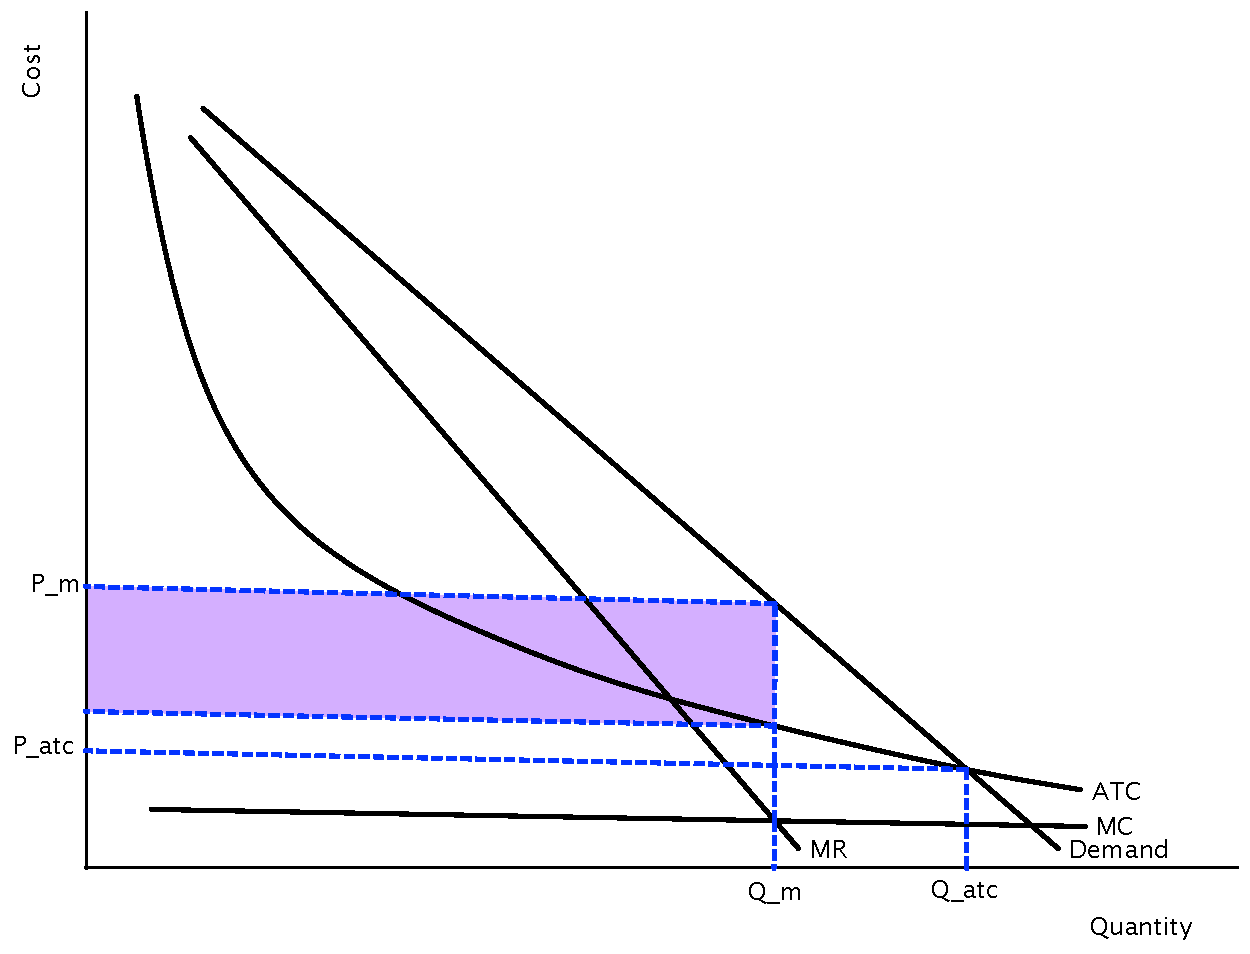
\includegraphics[scale=.18]{plot79.pdf}
					\caption{ATC Pricing}
				\end{subfigure}
			\end{figure}
		
		\end{enumerate}
\end{frame}

\begin{frame}{Readings and Assignments}
\begin{itemize}
	\item Today: Mankiw Ch. 15
	\item Next time: Mankiw Ch. 16 \& 17
	\item Problem Set 3, section 3
	\item Homework 3 due on 6/5
\end{itemize}
\end{frame}

\end{document}